\section{Theorie}
\label{sec:Theorie}
Unter Laserstrahlung versteht man hochintensive, monochromatische elektromagnetische Wellen. Diese Wellen besitzen eine hohe Kohärenzlänge.
Ein Laser (\textbf{L}ight \textbf{A}mplification by \textbf{S}timulated \textbf{E}mission of \textbf{R}adiation) besteht aus drei Komponenten. Diese sind
eine Pumpquelle, ein aktives Lasermedium sowie ein Resonator. Dabei sind Pumpe und das aktive Medium für die Erzeugung des Strahls verantwortlich. Der Resonator besteht aus zwei Spiegeln, die den erzeugten Strahl sowohl teils als
auch total reflektieren. Da so das Medium mehrmals vom Strahl durchlaufen wird, kann dieser stark verstärkt werden.
\subsection{Absorption und Emission von Photonen}
\label{sec:theorie1}
Es existieren drei wesentliche Wechselwirkungen für Photonen mit Materie, diese sind Absorption sowie spontane und stimulierte Emission.
In Abbildung (\ref{fig:3prozess}) sind diese schematisch dargestellt.
\begin{figure}[h!]
  \centering
  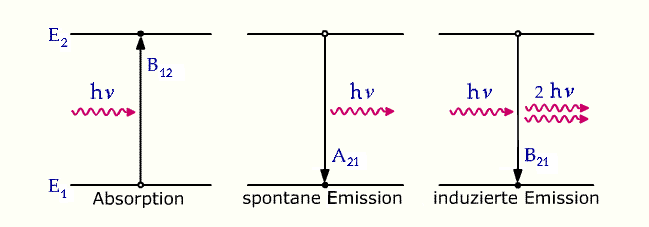
\includegraphics[scale=0.7]{fig/3prozess.png}
  \caption{Schaubild für die drei verschiedenen Prozesse \cite{Anleitung1}}
  \label{fig:3prozess}
\end{figure}
\subsubsection{Absorption}
Bei der Absorption wird ein Photon von einem Atom absorbiert. Bei diesem Prozess wird ein Elektron des Atoms in einen energetisch höheren Zustand angehoben, damit steigt die Energie des Elektrons und das Photon verschwindet.
Dieser Prozess ist nur möglich wenn die Energie des Photons $E_\mathrm{\gamma}$ größer ist als die Energiedifferenz zwischen Grund- und angeregtem Zustand $\Delta E$.
\subsubsection{Emission}
\label{sec:emissionen}
Befindet sich ein Atom nun in einem angeregten Zustand kann es auf zwei verschiedene Arten abgeregt werden. Der erste Fall ist hier die spontane Emission, dies kann als umgekehrter Vorgang zur Absorption gesehen werden.
Ein Elektron geht spontan aus einem energetisch höheren Zustand in einen energetisch niedrigen Zustand über, bei diesem Vorgang wird ein Photon emittiert mit der Energie $E=\Delta E$ der Energiedifferenz der beiden Zustände.
Der in diesem Experiment relevante Fall ist jedoch die stimulierte Emission, denn auf ihr beruht die Funklonsweise des Lasers. Bei der stimulierten Emission wird eine Abregung aus dem höheren Zustand durch ein eingestrahltes
Photon der Energie $E=\Delta E$ erzwungen. Dann wird zusätzlich ein Photon ausgesende, das in Richtung, Phase und Energie äquivalent zum eingestrahlten Photon ist. Die Photonen vermehren sich also wie in Abbildung (\ref{fig:3prozess}) zu sehen. Nur durch diese stimulierte Emission ist es möglich monochromatisches und kohärentes Licht zu verstärken und somit Laserlicht zu erzeugen.
\subsection{Erzeugung von Laserlicht}
Um Laserlicht mittels stimulierter Emission zu erzeugen muss im aktiven Medium eine Besetzungsinversion vorliegen, das heißt im energetisch höheren Niveau müssen sich mehr Teilchen befinden als im energetisch niedrigen Niveau. In einem
Zwei-Niveau-System ist dieser Zustand jedoch nicht, da dort die Teilchen auch bei beliebig hoher Intensität im höheren Niveau immer weniger sein werden als im niedrigen Niveau. In einem Drei-Niveau-System oder Vier-Niveau-System ist dies jedoch möglich, eine Vorrausetzung dafür ist eine hohe Intensität des Lichtes im Resonator. Dabei hat das Vier-Niveau-System den Vorteil, dass es unabhängig von der Intensität eine Besetzungsinversion erzeugen kann und somit sehr gut als Lasermedium genutzt werden kann. In Abbildung (\ref{fig:4niveau}) ist dies schematisch dargestellt:
\begin{figure}[h!]
  \centering
  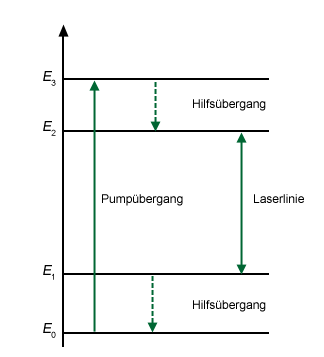
\includegraphics[scale=0.5]{fig/4niveau.jpg}
  \caption{Vier-Niveau-System \cite{Anleitung4}}
  \label{fig:4niveau}
\end{figure}
\FloatBarrier
In diesem Versuch wird ein Helium-Neon-Laser betrachet, dabei dient das Helium als Pumpe und das Neon als Lasermedium. Zunächst werden die Heliumatome in einen energetisch hohen Zustand gebracht. Durch Stöße zweiter Art mit den Neon-Atomen wird in diesen eine Besetzungsinversion erzeugt, somit ist es nun möglich stabil mit den Photonen mit der richtigen Energie dort die stimulierte Emission auszulösen und Laserlicht zu erzeugen. Durch die Spiegel im Resonator werden die ausgelösten Photonen wieder durch das Lasermedium geleitet und es kommt zu einem Kaskadeneffekt der die Photonen vervielfältigt.
\begin{figure}[h!]
  \centering
  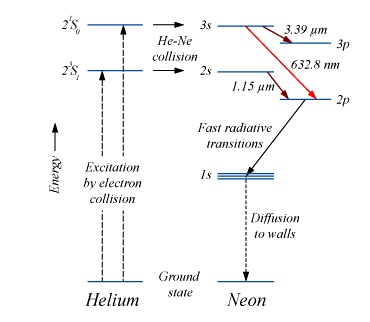
\includegraphics[scale=0.7]{fig/heliumneon.png}
  \caption{Funktionsweise des Helium-Neon-Laser \cite{Anleitung5}}
  \label{fig:heliumneon}
\end{figure}
Wie in Abbildung (\ref{fig:heliumneon}) zu sehen, ist der Übergang von 3s nach 2p der Neonatome für die rote Linie, das heißt Wellenlänge $\lambda=\SI{632.8}{\nano\meter}$, verantwortlich.
\subsection{Stabilitätsbedingung}
Damit ein einfacher Resonator wie im Helium-Neon-Laser als stabil gilt muss die Stabilitätsbedingung gelten, diese lautet:
\begin{equation}
  \label{eqn:stabi}
  0\leq g_\mathrm{1}g_\mathrm{2}\leq1
\end{equation}
Mit den sogenannten g-Faktoren:
\begin{equation}
  \label{eqn:g-faktor}
  g_\mathrm{i}=1-\dfrac{L}{R_\mathrm{i}}
\end{equation}
Dabei ist $L$ die Länge des Resonators und $R_\mathrm{i}$ die Krümmungsradien der Resonatorspiegel. Es gibt vier Grenzfälle, diese sind konfokale Resonatoren ($g_\mathrm{i}=0$), hemisphärische Resonatoren ($g_\mathrm{1}=0$, $g_\mathrm{2}=1$), konzentrische Resonatoren ($g_\mathrm{i}=-1$) und den sogenannten Fabry-Pérot-Resonator ($g_\mathrm{i}=1$).
\subsection{Moden}
\label{sec:modee}
Da die Resonatorlänge $L$ im  Vergleich zur Wellenlänge $\lambda$ sehr gro0 ist, erfüllen mehrere Moden die Stabilitätsbedingung. Die Moden werden $\mathrm{TEM}_\mathrm{lpq}$ berezeichnet. Dabei sind die Indize l und p die transversalen Knotenpunkte
in x- bzw. y-Richtung und q die longitudinale Mode. Die Mode $\mathrm{TEM}_\mathrm{00}$ heißt Grundmode und besitzt den größten Anteil am Modenspektrum ihre Intensität ist gegeben durch:
\begin{equation}
  \label{eqn:grundmode}
  I_\mathrm{00}(x)=I_\mathrm{0}\exp\left(\dfrac{-2(x-x_\mathrm{0})^2}{w^2}\right)
\end{equation}
Im Auswertungsteil werden ebenfalls noch die Intensitäten für die Moden $\mathrm{TEM}_\mathrm{01}$ (siehe Gleichung (\ref{eqn:01})) und $\mathrm{TEM}_\mathrm{02}$ (siehe Gleichung (\ref{eqn:02})) verwendet:
\begin{align}
  \label{eqn:01}
  I_\mathrm{01}(x)&=I_\mathrm{0}\dfrac{4(x-x_\mathrm{0})^2}{w^2}\exp\left(\dfrac{-2(x-x_\mathrm{0})^2}{w^2}\right) \\
  \label{eqn:02}
  I_\mathrm{02}(x)&=I_\mathrm{0}\left(\dfrac{8(x-x_\mathrm{0})^2}{w^2}-2\right)^2\exp\left(\dfrac{-2(x-x_\mathrm{0})^2}{w^2}\right)
\end{align}
\subsection{Brewsterfenster}
\label{sec:brews}
Damit das Licht möglichst verlustfrei austreten kann ist das Laserrohr mit Brewsterfenstern abgeschlossen, sie stehen dabei im sogenannten Brewster-Winkel zum Strahlengang. Durch die Brewsterfenster wird somit Licht, dass parallel
zur Einfallsebene polarisiert ist wesentlich verlustfreier durchgelassen als anders polarisiertes Licht. Dadurch wird die Polarisationsrichtung des emittierten Lichts festgelegt. In Abbildung (\ref{fig:brew}) ist dies dargestellt.
\begin{figure}[h!]
  \centering
  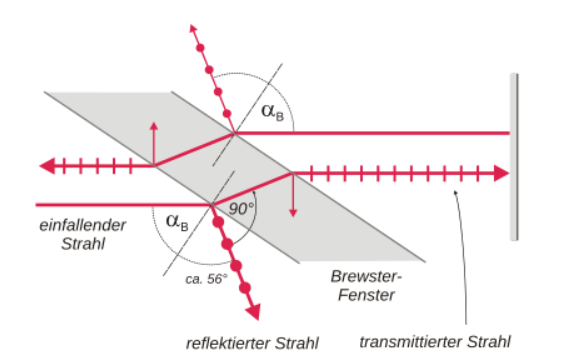
\includegraphics[scale=0.5]{fig/brew.png}
  \caption{Strahlengang am Brewsterfenster \cite{Anleitung6}}
  \label{fig:brew}
\end{figure}
